\chapter{Design and Implementation of Slope}
\label{chap:design}


We present the design and implementation of Slope, a migration framework which
satisfies the requirements and conditions discussed in the previous chapter.

\section{Design elements}
Slope has to provide features such as transferring objects without serialization
and deserialization that are rather unusual in more generic systems. We
therefore have to carefully introduce ideas to deliver these specific capabilities.

\subsection{Local memory layout}
\label{sec:localmem}
To eliminate the serialization and deserialization steps, we use a specific
memory layout to store migratable objects.
Similar to RAMP \cite{memon2018ramp}, each program instance reserves a
specific contiguous part of its virtual memory address space. The size of this
segment must be at least equal to the \emph{sum} of maximum physical memory that the
application plans to devote to migratable objects, this can be
as high as the total amount of physical memory in the cluster.
The starting address of this memory range is the same address on all machines.
This reservation is done at program construction time
(i.e. before \texttt{main()}).

We will refer to this section of the virtual
address space as migratable memory or Slope memory. Note that mappings for
these pages are not yet generated and therefore the size of the Slope memory
region can be expanded to the whole 64 bits of address on current machines.

To synchronize accesses to memory during the migration process, we need a way
to control accesses to the pages in Slope memory. We therefore choose to manage
Slope memory by 4KB page granularity as this is the smallest unit of control
for setting memory page protection mappings.

\begin{figure}[t]
\centering
\ensurepdffromsvg{local-memory-management-phys-log.drawio}
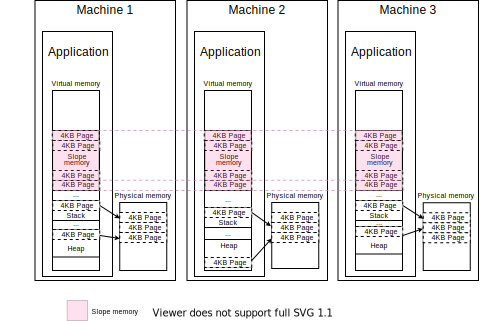
\includegraphics[width=1\textwidth]{local-memory-management-phys-log.drawio}
\caption{
    Placement of Slope memory on each node upon initialization.
}
\label{fig:localmemorymanagementphyslog}
\end{figure}

\autoref{fig:localmemorymanagementphyslog} shows how the local memory layouts
of the machines compare with each other. Notice how Slope memory is at the
same location in the virtual address space of the program on each node.
It also has the same size and page boundaries on all machines. Also note how
the 4KB pages from that region are not mapped to any physical memory pages
yet.

The placement of Slope memory in the application virtual address space is
central to the migration process. An object which only references addresses
within the Slope memory on one machine, can be moved to a different machine
and put on the same virtual address, page by page, along with the addresses
that it references and the object would continue to ``work'' in its new
residence. This in essence describes a migration operation and is how we will
eliminate the need to serialize and deserialize these objects.

This however requires multiple conditions to be in place, and multiple
housekeeping tasks to be taken care of. For example the object must not have
any references to resources falling outside of the migratable memory. These
could be objects in non-migratable memory, or file descriptors, which refer
to resources beyond the scope of the application. Memory allocation
and deallocation must be handled too to avoid objects from overwriting each
others' pages during a migration.

Starting from the local memory layout, all of the design elements and
sub-systems in Slope are directed towards providing a migration API with the
requirements discussed in the previous chapter, while enabling us to deal with
the above
issues.


\subsubsection{fundamental requirement of fixed addresses}
\label{sec:fixedfundamental}
\begin{figure}[tp]
\begin{lstlisting}
template<typename T> class ptr_hash;
template<typename T> class ptr_hash<T*> {
  using Type = T*;
 public:
  size_t operator()(const Type& ptr) const {
    return reinterpret_cast<std::uintptr_t>(ptr);
  }
};
int main() {
  std::unordered_map<int*, int, ptr_hash<int*>> m;
  std::vector<int> v(0);
  // v.reserve(2); // Uncommenting will result in passing the assert
  v.push_back(1); m[&v[0]] = 1;
  v.push_back(2);
  assert(*(m.begin()->first) == m.begin()->second); // fails
}
\end{lstlisting}
\caption{
    Referencing an object (int) through its virtual address
}
\label{fig:localmemorymanagementfundamental}
\end{figure}
It is important to note that although strict and inflexible, the requirement of
placing Slope memory on the same virtual address in all machines is,
unfortunately, a fundamental requirement. \autoref{fig:localmemorymanagementfundamental}
shows an example of why this is the case. It shows the creation of a hash
    function for pointers which simply uses their value, which is a virtual
    memory address. The vector needs to move the contents of its underlying
    array to a bigger array before inserting the second element. At this point, from the viewpoint of
    \texttt{m}, \texttt{v} has ``moved'', effectively shifting its start
    address to a new virtual address. \texttt{m} has no way of figuring out
    the new address and no way of translating its address dependencies.

In contrast, had the map stored indices instead of addresses, allowing them
to be translated to addresses internally in the map, this would not have been
a problem. \autoref{fig:refbyindex} demonstrates this. In this example,
the second call to \texttt{push\_back()} changes \texttt{\&v[0]}, however this
will not pose a problem since no object depends on it apart from \texttt{v}.

\begin{figure}[tp]
\begin{lstlisting}
int main() {
  std::unordered_map<int, int> m;
  std::vector<int> v(0);
  v.push_back(1); m[0] = 1;
  v.push_back(2); // results in v[0] being moved
  assert(v[m.begin()->first] == m.begin()->second); // succeeds
}
\end{lstlisting}
\caption{
    Referencing an object (int) through its index
}
\label{fig:refbyindex}
\end{figure}

The implication is as long as the
application has any means of referencing the underlying virtual address of any
of its resources, its correct execution may end up depending on that address
staying the same at every point during the execution of the program. Therefore
migrating an object without serialization and deserialization to another
machine (process)
requires byte by byte replication of its memory to the exact same virtual
addresses in the other machine (process) in the general case.

\subsection{Distributed memory management}
\label{sec:globalmem}
To simplify the discussion, from this point on we will assume that all of the
machines in the cluster have equal amounts of physical memory and that we want
to allow Slope to be able to use as much as all of the physical memory on each
machine.

Slope memory will therefore be of size $n \times m$ where $n$ is the number
of machines and $m$ is the physical memory available to each machine. We assign
the ownership of the first $m$ bytes of memory to the first machine, the
second $m$ bytes to the second machine and so on, such that the $i$th machine
owns the $i$th $\frac{1}{n}$ of Slope memory.

We can simplify the distributed ownership of memory if we only allow the
machines to allocate memory from the section that they own, however this may
result in memory address load imbalance. If one machine keeps
allocating objects and then quickly migrates them to the other machines. The
$\frac{1}{n}$ of the Slope memory belonging to this machine will soon run out,
and the machine will not be able to create any more migratable objects
even though the global Slope memory and the node's local physical memory are
far from full.

This requires us to devise a distributed memory management scheme which allows
us to use possibly all of the available Slope memory regardless of which
machine we are allocating the memory from, while avoiding clashes
between the allocated addresses across the cluster.


\begin{figure}[t]
\centering
\ensurepdffromsvg{leaserange.drawio}
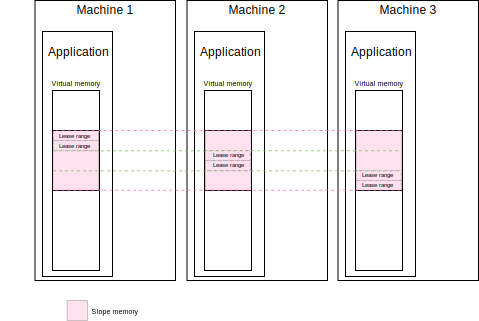
\includegraphics[width=1\textwidth]{leaserange.drawio}
\caption{
    Cluster memory layout and lease ranges
}
\label{fig:leaserange}
\end{figure}


We divide the Slope memory to sections that we call lease ranges. Each lease
range must be fully contained in one machine's $\frac{1}{n}$ of memory.
Lease ranges are the units of distributed ownership of Slope memory.
\autoref{fig:leaserange} shows placement of lease ranges
in slope memory.


At any point, each lease range is owned by at most
one machine. Initially, none of the leases are held by any of the machines.
For the duration of the program, each machine is responsible for
the leases that initially fall in its $\frac{1}{n}$ of Slope memory.
That means the machine can hand out
the lease ownership to itself or other machines for any of the leases it is
responsible for.


Machines allocate memory pages from the lease ranges they own. Initially when
the machines do not own any leases to allocate from, or when the unallocated
memory in the
ranges that they already own does not suffice for their new allocations, they
need to ask for a new lease. To solve the memory imbalance problem, each node
will locally decide to direct its request for a new lease to the machine which
has the highest number of free leases. Each machine broadcasts this information
to the cluster in long intervals. We set the lease sizes to be 1GB and
make each machine broadcast the number of leases it has available every 10
seconds.

The 1GB size allows for lease requests to be infrequent enough to amortize
seamlessly over the number of allocations, while keeping them small enough
to avoid sudden increases in the memory usage of any of the nodes. The 10
second interval keeps the lease ownership counts up to date across the cluster,
while causing little overhead to the application. However because of stale
information during the intervals, the nodes will not always
correctly choose the machine with the highest available lease count to allocate
from, but the 1GB size of the ranges which is relatively small compared to the
physical memory available to the machines will account for this inaccuracy.
This protocol
will keep the available number of leases in each machine roughly equal across
the cluster.

The above distributed memory allocation scheme not only eliminates the need for
a consensus box to track global memory allocations, but can also avoid
contention when multiple machines need to acquire new lease ranges with
little tweaks. For example each machine can randomly select to request the
lease from one of the top $k$ least occupied machines, instead of selecting
the least occupied machine, avoiding hotspots when multiple machine requests
for leases at the same time.

\subsection{Memory allocator}
\label{sec:platform}
The strict local and distributed memory requirements discussed in the previous
section suggest that we should manage the Slope memory using a custom memory
allocator. Since Slope requires intimate access to the application
memory, we need to choose a low level platform with first class support for
memory management.

We have chosen C++ as the platform to implement Slope, mainly because we need
to directly access process memory and manage the way it is allocated and used.
We implement \texttt{slope::memory::Allocator<T>} which is a memory allocator
conforming to the C++ allocator name requirement (e.g. providing
\texttt{allocate()} and \texttt{deallocate()}). It will internally satisfy the
local and global memory requirements of Slope following the protocols discussed
in \autoref{sec:localmem} and \autoref{sec:globalmem}.

\begin{figure}[t]
\begin{lstlisting}
using MigratableUserDefinedType =
    UserDefinedType<T, slope::memory::Allocator<T>>;
\end{lstlisting}
\caption{
    Making predefined types migratable
}
\label{fig:migratableuserdefined}
\end{figure}

Any C++ type which accepts an allocator and uses it for all of its memory
allocations (i.e. \texttt{AllocatorAwareContainer} named requirement in the standard)
can be passed Slope's allocator. \autoref{fig:migratableuserdefined}
demonstrates how a preexisting well written user defined type can be
passed Slope's allocator without the need to change its internal implementation.

\begin{figure}[t]
\begin{lstlisting}
template<
    typename T,
    typename Allocator = std::allocator<T>
> class vector;
\end{lstlisting}
\caption{
    Declaration of \texttt{std::vector<T>}
}
\label{fig:stdvector}
\end{figure}


\begin{figure}[t]
\begin{lstlisting}
template<typename T>
using migratable_vector = std::vector<T, slope::memory::Allocator<T>>;

\end{lstlisting}
\caption{
    migratable \texttt{std::vector<T>}
}
\label{fig:migvector}
\end{figure}


With this design decision, STL containers (except \texttt{std::array} which
does not satisfy \texttt{AllocatorAwareContainer}) alongside many other preexisting
C++ structures can be easily made migratable.
For example \autoref{fig:stdvector} shows how the declaration of
\texttt{std::vector<T>}
allows the user to pass a custom allocator type. \autoref{fig:migvector} shows
how we can use the pattern in \autoref{fig:migratableuserdefined} to create
an alias for migratable vectors.



\begin{figure}[t]
\begin{lstlisting}
template<typename T, typename Allocator>
class UserDefinedType {
    static inline Allocator allocator;
    std::vector<T, Allocator> vector_;
    T *ptr_;
 public:
    template<typename... Args>
    UserDefinedType(Args&&... args):
      ptr_(new (allocator.allocate(1)) T(std::forward<Args>(args)...)) {}
    // ...
};
\end{lstlisting}
\caption{ Partial implementation of \texttt{UserDefinedType} which accepts an allocator}
\label{fig:userdefinedtype}
\end{figure}


A possible implementation for the \texttt{UserDefinedType} shown in
\autoref{fig:migratableuserdefined} might look like \autoref{fig:userdefinedtype}.
The class uses the allocator type passed to it to carry out any memory
allocations. Notice how the allocator can be conveniently passed down to the
class members (e.g. \texttt{std::vector<T, Allocator>}), showing the
composition-friendliness of using allocators classes that conform with C++ named
requirements.











\subsection{Memory ownership tracking}
\label{sec:ownershiptracking}
Passing Slope's memory allocator to types is not enough.
When an object is migrated to a different machine, we need to move all of the
memory that it references to the destination machine and put them at their
corresponding virtual memory addresses. This means
that we need a mechanism to keep track of the memory that an object owns.

We manage migratable objects through migratable pointers. The template\\
\texttt{slope::memory::mig\_ptr<T>} represents these types. A migratable
pointer works very similarly to a \texttt{std::unique\_ptr<T>}, with the
main distinction that it provides methods through which we can keep track
of the memory allocated by the underlying object. Furthermore after the
migration, we can recreate the underlying object of type \texttt{T} from
the migrated memory pages into a \texttt{slope::memory::mig\_ptr<T>}.

Most importantly, a migratable pointer provides a \texttt{create\_context()}
method which we must use to inform Slope of any memory allocations.
\autoref{fig:migptrusage} shows an example usage of this. For any method call
on type \texttt{T} that underlies the \texttt{slope::memory::mig\_ptr<T>},
if it has a possibility of calling \texttt{allocate()} on Slope allocator, it
must be enclosed in a context. We call this behavior ``allocating memory for
an object''.

\begin{figure}[tp]
\begin{lstlisting}
using HashTablePartition = DistributedPartition<
    int, // key type
    int, // value type
    slope::memory::allocator<int>
    >;

int main() {
    int key = 1, value = 2;

    // underlying type uses slope::memory::Allocator
    // default constructor of HashTablePartition is used
    slope::mig_ptr<HashTablePartition> ptr{};

    {
        // method called on mig_ptr
        auto context = ptr.create_context();

        // method called on the HashTablePartition through operator&
        ptr->put(key, value);

    } // context is invalidated as it goes out of scope
      // and destructor is called

    // No memory allocation possible; no context required
    ptr->get(key);
}
\end{lstlisting}
\caption{
    usage of \texttt{create\_context()} method
}
\label{fig:migptrusage}
\end{figure}


We keep a stack of contexts as they are created and destroyed by the application.
At each call to \texttt{allocate()}, the \texttt{mig\_ptr} whose context is at
the top of the stack will be set as the owner of the allocated memory.

Another important purpose that the \texttt{mig\_ptr} class template serves is
constructing the object itself. In addition to the memory allocations done
\emph{by} the object (e.g. allocating the underlying array by \texttt{std::vector}),
the object memory itself (\texttt{std::vector} object) must be placed in
migratable memory. This is an important step since we are not necessarily able
to construct the object elsewhere and then manually move it into the migratable
memory.

\subsection{Ownership management summary}
We will go over an example scenario to show how different layers of memory
ownership work together. Take the code snippet from \autoref{fig:migptrusage}
and assume it is being run on machine 1, in a cluster consisting of 3 machines.
Here is a possible course of events that we may observe on this machine.

First, the migratable pointer is created in \emph{non}-Slope memory. The
migratable pointer is only responsible for holding onto the migratable object
and does not need to be migratable itself. It will in turn try to allocate
Slope memory equal to the size of a \texttt{HashTablePartition} and constructs the
hash table in that memory.

Before the call to \texttt{allocate()} it creates
a temporary initialization context which we will later point to the object
that is about to be created. This is required because there is a circular
dependency between allocating the memory on which we are constructing the
hash table and setting the owner of that memory to be the hash table itself.
The circular dependency arises because we are not aware of the address of the
hash table before we allocate its memory.

After creating the initialization context, we call into \texttt{allocate()}.
Machine 1 does not yet hold any lease ranges, so it will try to ask for one.
After looking at the current number of available lease ranges at each node,
it will choose one of the three nodes in the cluster at random since all of them
have an equal number of available lease ranges. Machine 2 will be selected and
the request for a new lease will be sent to it by Machine 1. After being given
the ownership of a lease range by Machine 2, we continue in the
\texttt{allocate()} function. We now have 1GB of Slope memory available on
machine 1.

We then allocate a page from the newly owned lease range (assuming the size of
a \texttt{HashTablePartition} is much less than a single memory page), and assign the
page and the allocated memory inside the page to the object that is being
created by breaking the circular dependency which is described above.
We return from the \texttt{allocate()} function and the initialization context
will be removed from the context stack.

We return from the constructor of the \texttt{HashTablePartition} and then
the migratable pointer. The call to \texttt{create\_context()} on line 16 
will place
\texttt{ptr}'s context at the top of the context stack. As a consequence, all of the
Slope memory allocations will be assigned to \texttt{ptr} until further change
to the context stack. We call into the \texttt{put()} member function, which
results in a call to \texttt{allocate()}. More memory will be allocated from
the page that embodies the \texttt{HashTablePartition} object since that page
still contains some empty space. With its context present at the top of
the context stack,
\texttt{ptr} will own the newly allocated memory. Afterwards the context will
go out of scope, resulting in \texttt{ptr}'s context being removed from the
context stack, leaving it empty.
The call to \texttt{get()} will not invoke any of the Slope functions.

It is important to note that allocated memory is not necessarily mapped to
physical memory. As an example if the \texttt{ptr} object from
\autoref{fig:migptrusage} is migrated to Machine 3, its underlying memory
will remain allocated from the standpoint of Machine 1 which is responsible for
the lease lease range under \texttt{ptr}.
However Machine 1 will unmap those memory pages after the migration.
In contrast, on Machine 3, those pages will indeed be mapped to
physical memory after the migration.

\section{RDMA background}
RDMA programming model turns out to be a good fit for the networking
requirements of Slope. While we do benefit particularly from
offloading data plane processing from the source CPU to the network device,
RDMA networking can still be swapped out of Slope for other transports.

To send or receive data using kernel-based TCP, the application needs thread
is woken up multiple times by the kernel and has to call into the kernel
repeatedly, copying all of the payload between user and kernel space buffers.
RDMA networking prevents this by 1. allowing data to be sent/received without
the need to copy it from/to a temporary buffer, and 2. not calling into the
kernel on the critical path.

The following paragraphs introduce several concepts in RDMA
networking from control structures to Infiniband verbs. To keep this section
concise and on-point, we mostly describe the Infiniband features that are used
in Slope and skip low level details such as the role of various configuration
variables in the setup process.

An Infiniband subnet consists of hosts and switches that are interconnected
through their Infiniband adapters or Host Control Adapters (HCA).
Each subnet requires at least one Subnet Manager (SM) to function.
Infiniband switches or end hosts may play the role of SM. Multiple SMs
work in Active-Stand by mode. Among more complicated tasks such as managing
routing throughout the local subnet and possibly through the global Infiniband
Fabric, one of the responsibilities of the SM is assigning unique local
identifiers (\texttt{lid}s) to each port connected to the current subnet, not much
different from how a DHCP server assigns unique IP addresses to each device
that is connected to an IP network.

Queue pairs (QPs) can be thought of as being analogous to sockets in TCP/IP
networking. In our case we only use the reliable connected (RC) type of queue
pairs which guarantees reliability and in-order delivery.
A QP logically ``connects'' two hosts so that they can communicate using
RDMA verbs. Each of the two hosts independently creates a QP structure. The
QP is assigned a locally unique \texttt{qp\_num} to distinguish between the
QPs on the same host. The two QP structures then have to be introduced to
each other by transitioning them through multiple states, namely init, ready to
receive, and ready to send.

At certain points during these transition, each
QP end needs to know about the \texttt{lid} of the remote Infiniband port to
be able to identify and reach that port through the subnet. Naturally the
remote \texttt{qp\_num} has to be known for each QP end to be able to
distinguish and correctly select the target QP end's \texttt{qp\_num}.
Applications need to improvise their own methods of exchanging these two
pieces of information, typically called the out of band rendezvous and ready to
send protocols. We use memcached for this where every participating machine
registers the \texttt{lid} and \texttt{qp\_num} corresponding to each of its
QPs, alongside the intended remote node of this QP under that machine's key.
The number of machines and their registration keys
are known at the execution time of the program by all instances. After
publishing their information each machine goes through the keys corresponding
to other servers and blocks until finding their QP information in memcached.
After that each server $S$ selects the QPs whose intended remote node equals
$S$ and with the \texttt{lid} and \texttt{qp\_num} of that QP at hand, it
transitions the QP through the required states to make it ready to use. This
only happens at the initialization of the cluster after which we never use
the memcached instance again.

From this point on, each machine can use any of its QPs to exchange data with
the other end of the QP through the use of RDMA verbs. The QP APIs are
asynchronous, meaning the application calls into the Infiniband library to
``posts'' operations to the QPs, and ``poll'' the completion of certain events
such as the completion of a send request.

To send data using the RDMA SEND verb, the application needs to ``post'' one
or more send Work Requests (WRs) to the send queue of a QP. Among other fields
to control its behavior, a WR is consisted of one or more
continuous memory ranges that need to be sent through a QP. Each of these
is called a Scatter-Gatter Element (SGE). However the network device must be
able to access the memory pages that the SGEs point to through their physical
addresses, and those physical addresses must not change throughout the time
that the SEND is in progress. To make sure that is the case, the addresses
that underlie the SGEs must be subsets of Memory Regions (MRs) that we
explicitly register with the Infiniband library. Creating an MR from a set of
continuous memory pages will pin them in memory until the MR is
deregistered. To process the SEND request, the network device might reference
addresses from MRs that the SGEs point to, until that particular WR is
processed which means we are not allowed to write to those regions during
the time SEND is being processed. By default, a successful SEND request will
create a CQEs upon completion. The application can be notified of the completion
of the SEND WR by polling the CQ that is associated with the QP. After receiving
the completion, the application is free to deregister and/or write to the
memory under the MR.

For a SEND to succeed, the destination must have previously posted a suitable
RECV request to the Receive Queue of its end of the QP. Similar to the case with SENDs,
a RECV request takes the form of one or more receive WRs each of which
consists of multiple SGEs, which point to local memory that is pinned using
MRs. At the receiver, this will result in the data from the SGEs of the incoming
SEND to be written by the network device to the memory addresses that the
receive WR specifies through its SGEs.

Together, SEND and RECV are called two-sided verbs, meaning they require
intervention from both the sender and the receiver. In contrast, the one-sided
READ and WRITE verbs completely bypass the remote machine's processor and do not
produce entries in the CQs of the remote machine. To
issue a READ or WRITE, the caller must first pass SGEs referring to local memory
from which data will be READ, or to which data will be written, respectively.
In each of the above we must also specify an address in the remote machine
as the source for READ or the destination for WRITE. This address is in
the virtual address space of the remote machine, and must be contained in an
MR. The caller also needs the know the remote key (\texttt{rkey}) of the target
MR in the remote machine. Similar to the case with \texttt{lid} and
\texttt{qp\_num}, the application has to arrange for the \texttt{rkey} to be
transferred to the caller before it can call one sided VERBS. However with the
QPs now established, we do not necessarily need to rely on an out of band
communication mechanism to hand off \texttt{rkey}s as they can be sent using
RDMA SEND and RECV verbs.

We also use a variant of WRITE called ``WRITE with immediate values'', which
differs to a WRITE in that it generates a completion in the CQ of the
remote QP.

To know about which operations have been completed, applications must poll the
Completion Queue (CQ) structure.
Each QP is associated with one CQ. Applications may decide that some of their
QPs share a single CQ to reduce the number of separate structures that they
have to poll. As a result of polling the CQ, the application is handed
Completion Queue Entries (CQEs) which reveal the source of the completion.


\section{Architecture}
At a high level, Slope consists a control plane, responsible for carrying out
different phases of the migration operation and provide the means for the
servers to send and receive metadata to eachother, a data plane, in this case
over RDMA which handles sending and receiving memory pages,
and a specialized distributed memory management scheme, described earlier in the
chapter. Slope's migration protocol is built atop the above sub-systems.

% We have implemented the control plane and the data plane using
% RDMA over Infiniband because of how well the benefits of RDMA networking
% fit our problem specifications, but they can be implemented using any transport.

\subsection{Control plane}
The control plane provides an abstraction over which application instances can
execute migration operations and other side-tasks such as exchanging internal
system metadata or distributed memory allocation. For each operation we create
a reliable connected queue pair between each pair of machines, and pre-post to
them as many receive requests as we need to support concurrently. When a
machine pulls out a work completion from the completion queues assigned to
these queue pairs, a receive buffer is reposted to the corresponding queue to
make up for any other incoming requests, and a request flow starts during which
the two machines will go back and forth to carry out the operation.

% Although
% the control plane can be practically replaced by any rpc framework, we do not
% have much to gain from using systems such as Herd \cite{kalia2016designguidelines} or
% FaSSt \cite{kalia2016fasst}, as the performance metrics in Slope are dominated
% mostly
% by the performance of the data plane.



% When using connected queue pairs, meta-data
% from each queue has to exist on the device cache for any operations to be
% carried out through that queue pair. As the number of queue pairs on each node
% increases linearly with the number of nodes in the cluster when we connect the
% QPs in a full-mesh manner, the performance of the application will collapse
% after we pass a certain number of nodes in the cluster, which has
% incentivized designs of RPC systems that use datagram queue pairs such as
% \cite{kalia2019datacenter} and \cite{kalia2016fasst}, even though others such
% as \cite{novakovic2019storm} have proposed hybrid one sided and two sided
% schemes which scale well. We have not reached a point where we can directly
% benefit from these optimizations as we are mostly throughput (data plane)
% limited. Furthermore we use each queue pair repeatedly in short bursts after a
% migration operation is triggered which avoids invalidating the ``active'' QP
% meta-data from the cache during the migration. However the control plane
% can be replaced entirely with any other RPC mechanism that achieves better
% performance.

% For co-ordination between machines (e.g. rendezvous protocol and transition
% to ready to send state)
% an out of band communication mechanism has to be used. We use memcached where 
% every node registers its queue pair and memory region parameters and
% information and waits to receive the same information from its peers. This
% phase only runs early in the program and does not have an effect on the
% performance of the system after the initialization is finished, at which point
% we no longer need the memcached server.

\subsection{Data plane}
The data plane is used to transfer contents of pages of Slope
memory from one machine to the same page addresses in another node. As we
will see when discussing the migration protocol, the data plane is used
in two separate phases called \emph{prefill} and \emph{transfer}. The prefill
phase sends the pages of a migratable object to the destination with
relaxed consistencies, and is followed by transfer, which ensures that the
object is sent correctly and is in a valid state at the destination.

% relaxed consistency requirements. Transfer operation follows shortly, during
% which we ensure the contents of the above memory section in the source are
% replicated to the same virtual addresses on the remote node. Prefilling is done
% in 4KB page granularity, while transfer can be done in larger units, depending
% on the contiguity of the memory section that is being transferred.


\section{Migration protocol}
\label{sec:migrationprotocol}

\autoref{fig:migrationprotocol} outlines the migration protocol and the role
of Slope at different stages during the above timeline.

\begin{figure}[tp]
\centering

\ensurepdffromsvg{migration-protocol.drawio}
\includegraphics[width=1\textwidth]{migration-protocol.drawio}
\caption{
    Slope migration protocol starting from object creation. Time progresses
    downwards.
}
\label{fig:migrationprotocol}
\end{figure}

We observe the lifetime of a migratable data structure from the point it is
created until after we finish migrating it to another node. As discussed
later in the section in detail, throughout the
there are certain conditions that need to be satisfied by the application
for the migration operation to finish correctly.

\subsubsection{Object creation}
During this phase the source machine calls into the Slope library multiple
times, based on how many times memory allocation and deallocation is required.

\paragraph{Source} creates a migratable object. Let us call this object
the target object. Up until the point that
the source initiates the migration, all of the memory allocations of the target object
must happen through
Slope's custom memory allocator through allocation contexts as discussed in
\autoref{sec:ownershiptracking}.
The application must enclose the memory allocations of the migratable objects
with the correct allocation contexts to make sure Slope correctly keeps track of the
memory that each object references.

After the object is created the program will call the \texttt{run()} method
of the object, which may result in further calls to the memory allocator as
the object might need to allocate memory to process its incoming requests or
carry out the calls to its member functions. These new allocations will be
correctly picked up by Slope allocator given that allocation contexts are used,
meaning at any point in time we know which memory pages belong to the target object.

\subsubsection{Migration initiation}
The application logic decides that the target object must be migrated from the
source machine to the destination. This might happen because the source machine
is balancing out its load by offloading the object to the destination or because
this particular object will benefit from running on the destination machine
by being local to resources that are available there.

This is the first time that the destination
machine will need to know about the properties of the target object. Had the
source machine not initiated the migration, the destination machine would have
stayed unaware of the existence of this object.

\paragraph{Source}
initiates the migration by calling into Slope. From this point
on, the application instance on the source machine is neither allowed to
cause any memory to be allocated to the target object, nor can it deallocate any memory that
this object references. Each of these can result from calling member functions
of the target object which either deallocate Slope memory previously held by the
object, or create Slope memory allocation contexts from the object and
use them to allocate Slope memory for the object.

This means the underlying Slope memory owned by this object is now
fixed. The application can continue to read or write to the memory that the
object already owns, until further on in the process when it receives a
notification from the Slope library. This notification signals that source
machine no longer owns the object, prohibiting this machine from any
interaction with the target object, including reading from or writing to its
memory. This will be discussed in detail in the following sections.

Slope posts a send request to the QP that is shared
between the source and the destination, initiating the migration.
With this request, the source will include $n$ the total number of
memory pages that the target object references. Note that Slope requires the
memory pages owned by the target object to stay the same during the migration
process after a call which initiates the migration, which means $n$ will be
constant throughout the process.

\paragraph{Destination}
receives a migration request along with $n$, the number of memory pages that the
target object owns and therefore need to
be transferred. The destination then populates another QP shared with the source
with $n$ receive requests, each corresponding to one of the virtual memory pages
that underlie the target object. We switch to a different QP
to allow concurrent migrations to happen between pairs of nodes. The destination
then goes on to notify the source that it can receive the description of the $n$
pages. The destination needs to know the page addresses
to first create mappings for them and then pin them in physical memory so that their
physical address will stay the same throughout the migration, while the network
device writes to the pages by their physical address over DMA.

\paragraph{Source} receives the clear to send from the destination and sends the starting address
of each of the $n$ pages to the destination. 

\paragraph{Destination} waits for $n$ page addresses, and for each one of them, pins the
corresponding page in physical memory, so that the addresses that underlie the
target object can be used in RDMA read and write verbs. Notice how
``pro-active'' strategies which do not require knowledge of the page addresses
will not work, as pinning the
whole Slope memory in the physical memory will in the worst case, exhaust the
available physical memory on some nodes, and in the best case, result in large
amounts of wasted physical memory space. When the $n$ pages are pinned
and are ready to be the target of the RDMA verbs, the destination responds back,
signaling that it has pinned all of the required pages.

\subsubsection{Prefill}
The goal of the prefill phase is to warm up the destination machine's memory to
minimize the window of time during which none of the two participating machines
own the target object. No machine can read from or write to the object during
that time. Therefore a long window without no owners means a long throughput
and latency hiccup as the application does not make any progress.

During the prefill phase we copy the target object to the destination over RDMA.
What makes it different from simply transferring the contents of memory is that
during the prefill operation, the source is still allowed to write to
any location in the target object memory,
despite not having permission to change the memory layout of the object
in any way by allocating or deallocating memory. We optimistically do the above
transfer knowing that some of the pages might need to be retransferred as they
are written to by the source machine after they are sent to the destination.
We will refer to these pages as dirty pages. While pages can be
dirtied, we go through the prefill phase, hoping that one of the
machines (namely the source machine) will be able to partially function during
this phase, while dirtying a small percentage of the pages.

\paragraph{Source} will need to loop through the memory pages of the target
object to prepare them to be read safely by the network device. It will then
need to use RDMA WRITE to send them to the destination, but before it is ready
to go through these, it must put in place the means to detect the pages that
are dirtied. A page will be dirtied when a write takes place in it, after
it is sent to the destination.

\subparagraph{Dirty page detection:}
This will be done using memory mapping protections and manually
handling signals that
are raised as a consequence of accesses to the protected memory pages.

First, the source overrides the default behavior of handling the
\texttt{SIGSEGV} signal using a call to
\texttt{sigaction}, to prevent the program from terminating on invalid memory
references. It is important to keep in mind that \texttt{SIGSEGV} is delivered
to the \emph{same} thread whose current instruction reads or writes memory
from a page that does not have the required permissions.

To synchronize the access to the pages of the target object,
we set the protection flags of each page to \texttt{PROT\_READ} before sending
it over RDMA. This prevents any writes from happening while RDMA WRITE
is in progress. These writes will result in a \texttt{SIGSEGV} signal being
raised because of an invalid memory reference, and the thread will start
executing our custom \texttt{SIGSEGV} handler.

Inside the signal handler, we make note of the address the access
to which caused the signal to be raised. This can be found in the
\texttt{si\_addr} field from the
\texttt{struct {*}siginfo\_t} which is passed to the handler.
Assuming this is an address in a
page that the target object owns, we mark the page containing the address as
dirty. In the simplest case, the RDMA WRITE corresponding to this page has
previously finished. We update the protection flags of this page back
to \texttt{PROT\_READ | PROT\_WRITE}
to allow further writes to the addresses in this page to succeed.

Otherwise the RDMA WRITE is still in progress in which case we need to be
more careful. In this case we need to wait for the
RDMA WRITE to finish before adding the \texttt{PROT\_WRITE} permission flag to
the page. In our
implementation we use a conditioned shared mutex where the thread which carries
out the RDMA operations is the writer and the threads that may call into the
signal handler are potential readers. As a result, each thread will will block
inside the signal handler until
the address to which they are trying to write acquires the correct permission.
\autoref{fig:dirtydetection} shows the execution flow of multiple threads
as each of them they fall into one of the above cases while Slope prefills a
page.

\begin{figure}[tp]
\centering

\ensurepdffromsvg{dirty-detection.drawio}
\includegraphics[width=1\textwidth]{dirty-detection.drawio}
\caption{
    Execution flow of different application threads during the migration of
    the 4KB page at \texttt{0xc000} which at some point in time becomes dirtied.
    Time progresses downwards and the prefill has been started before all of
    the events in the figure. Notice how thread t2 coincidentally never
    deviates from its happy path.
}
\label{fig:dirtydetection}
\end{figure}

\subparagraph{Preparation:} At this point in the process, the source still
has ownership over the target object memory. This means we need to coordinate
the access to these pages to prevent simultaneous reads and writes. To do this,
the source uses \texttt{mprotect} to make the current page read-only.
Semantically, the application is still allowed to write to the current page,
except when the RDMA SEND is happening.

\subparagraph{Send:} Each page is posted to a data plane QP shared between the
source and the sink, to be written to its corresponding virtual address in
destination over RDMA. Notice that we do not put the \texttt{PROT\_WRITE} permission
of the current page back after the RDMA SEND finishes, as we need to
detect any future writes which will dirty the page.
However we do set a condition variable which a threads running the signal
handler will check to know whether or not it is clear to put the \texttt{PROT\_WRITE} flag back.
At any point in time the clean pages will have their condition variable unset,
which is how we distinguish between the dirty and clean pages.

One by one, the source prepares and writes each page that the target object
owns, using the above procedures and keeps track of which of them is dirtied
over time.

\subsubsection{Transfer of ownership}

Contrary to case of detecting the pages that become dirty, which can be done
as described above, prevention of this phenomenon cannot be dealt with this way.
For example we may try to set \texttt{PROT\_NONE} permission on a page to
prevent accesses to it after we have started to send it to the destination.
The reason why this will not work will be discussed in the next section.


This cannot be correctly enforced by means such as setting the
\texttt{PROT\_NONE} on these pages. First, we might need multiple
\texttt{mprotect} calls to accomplish this if the pages are not adjacent,
meaning that we cannot assume the access to the object is ceased at a single
point in time. Furthermore even if we are able to take away the access to all
of the memory under the target object at once, if an application thread is
currently in the process of writing to the above memory, there is no right
action we can take from outside the application. For example this might have
been one write operation in the middle of a series of writes that the
application had been doing during the execution of a certain function.
Therefore
from the standpoint of the library, we do not have enough information to deal
with cases similar to these, as aside from detecting the illegal writes, there
is no right action to take to remedy them.

\label{sec:transferownership}
At this point we are ready to turn the ownership over to the destination.
We also have to notify the application at the source to stop referencing the
target object for both reads and writes before we can proceed.

\paragraph{Destination} receives the completions for the prefill RDMA WRITEs.
That is because those WRITEs are done with immediate values which will results
in completion entries to be created for them. After the destination
receives the completion of the
last SEND, it will send a request back to the source, asking the source to
finally give up the ownership of the object.

\paragraph{Source} calls back to the application upon receiving the above
message to make sure the application will not reference the target object
for either of reads or writes after the callback returns. The application is
therefore responsible to block the callback an notifies all of its threads to
finish their ongoing operations on the target object. The application will
ideally transition to a ``pre-transfer'' mode after the initial migration
initiation. In this phase the application will try to do mostly read-only
accesses to avoid dirtying too many pages as this will cause the migration
to be done less efficiently with more pages that need to be transferred twice.
\autoref{sec:api} discusses this in detail and \autoref{sec:conform} will
discuss how this model fits naturally in C++ programs.

After the application clears the migration, effectively promising to never
reference the target object again, Slope will use the dirty
page tracking data to identify the dirty pages and send their addresses
to the destination. This message will also hand over the ownership
of the target object to the destination.

\paragraph{Destination} is notified that it has been given the ownership of
the object and is clear to start the \texttt{run()} method of the object,
but also needs to re-pull the dirty pages whose address is attached to the
request since the contents of these pages on the destination machine are
outdated.
Slope starts the above two processes concurrently. The destination machine
first sets
\texttt{PROT\_READ | PROT\_WRITE} access for the clean pages and
\texttt{PROT\_NONE} for the dirty pages. We put the dirty page addresses into 
a priority queue and fetch them from the source machine in order, giving
precedence to the pages which result in a
\texttt{SIGSEGV} being raised at the destination from an access by the
application. This means that the page has \texttt{PROT\_NONE} permission set and
is immediately required by an application thread. When the page is pulled using
RDMA READ, the page mapping flags will be updated to include read and write
permissions and any thread waiting for those pages can proceed. This is done
similar to how we do the dirty page detection on the source machine which was
discussed earlier.

\subsubsection{Post-transfer}
After the transfer is done, the state of the application will be
indistinguishable from a situation where we allocated the target object on
the destination machine from the start, if we deal with one final housekeeping
task.

\paragraph{Destination} will notify the source that it has READ all of the
dirty pages and that it no longer needs the destination to keep the
pre-transfer content of the object memory.

\paragraph{Source} will wait to receive the above message at which point it
safely \texttt{munmap}s the memory underlying the ``old'' target object. At
this point the state on the source looks as if the said object had never existed
there.


\section{Optimizations and Corner cases}
Multiple optimizations opportunities and housekeeping tasks have been omitted
from the earlier parts of this chapter. In this section we attend to these
subtle but important left out pieces.

\paragraph{C++ programming style to account for the prefill phase}
\label{sec:conform}
Writing programs that can both respect and leverage the prefill phases
described previously is important to keep code readable. We can encode the
conditions and requirements of the migration phase using C++ language features.
For example to represent the object after the prefill phase starts, we can
stick to using only a \texttt{const} reference to the target object,
forcing the user to use a discouraged \texttt{const\_cast} to be able to call
into the type's non-\texttt{const} methods.

\paragraph{Allocation strategies:} There are multiple ways to improve the memory
allocation performance. Since we need to allocate memory to objects in page
granularity, it is important to reduce fragmentation and wasted space,
otherwise the two will quickly pile up to decrease usable memory and increase
communication overhead. One optimization towards preventing this is to allocate
new memory from the page(s) that an object already owns instead of adding
new pages to an object every time \texttt{allocate()} is called on behalf of it.

Applications may want to provide their custom allocators on top of the Slope
allocator which allocates big regions from the shared address space. Given the
above note, using a general
allocator inside Slope would not be meaningful since internally, Slope's
allocator is optimizing towards a specific and object-local goal (namely
reducing the number of pages that an object owns) compared to the usual
global object-agnostic goals of generic allocators.

However it might
nevertheless be helpful to allow applications to pass in their own solutions
to the former problem. For that matter, general allocators' approaches can
be reused. For example we can pose the problem of ``fitting a new allocation
into one of the part-filled pages of the current object'' to a user supplied
allocator.

\paragraph{Deallocation:} Reasoning about and implementing deallocation must
be done with care since we have a local and a distributed level of memory
allocation in the system and multiple problems must be dealt with.

We need to handle deallocations both locally and globally. More concretely, we
need to correctly make note of the deallocated memory of each object, and also
keep track of the usage of each range lease such that they can be handed back
to their owners when they are no longer required.

Deallocation does not require an active context. Notice that requiring
an active context during deallocation is out of the question, since
deallocation could be happening in an object's destructor. This does not pose
a problem since we can keep an inverse map from memory allocations to
migratable objects and update it at each call to \texttt{allocate()}. We can
then use the inverse map to correctly attribute each deallocation with its
respective object and update the pages that underlie the object if necessary.

When a machine deallocates memory referenced by a migratable object, this
information needs to be sent back to the lease holder of the memory range in
which the deallocated memory falls. We do this off the critical path, such that
each meachine accumulates deallocated memories and sends them in batches to
the machines that they originally belonged ($i$th $\frac{1}{n}$ of the
shared address space originally belongs to the $i$th machine), since the machine
on which the
deallocation happens does not have any information about
the actual lease owner of the embodying memory range. The original owner
of the memory range is then responsible to relay this information to the current
lease holder.

The timings of these requests do not pose a problem. That is
because while deallocations can happen globally, allocations from a memory range
happen only at the owner and the order in which we interleave the two types of
operations cannot result in double deallocation (since each object is owned by
exactly one machine) and double allocation (since all of the allocations happen
at the current node on unallocated memory). The lease holder can turn the lease
over to the original owner if it does not contain any allocated memory.

\paragraph{Optimizing communication over RDMA:} There is room to optimize
the RDMA communication further. In some steps during the migration, we
increase the smallest unit of communication from pages to continuous chunks
of memory, possibly spanning multiple pages. Similarly when calling for
READs/WRITEs on continuous chunks or pages, we chain together multiple
WR's and post them in a single request to decrease the number of times we
have to notify the network device using MMIO over the PCIe bus.

In the prefill phase, instead of sending the full list of dirty pages to the
destination so that it can prioritize which of them to READ first, we can
proactively choose one or a small number of the pages and WRITE them in
parallel to sending the dirty list to the destination to save half of an rtt
in latency and leverage the free bandwidth.
For example we can prevent one page fault on the destination
if the page in which the allocated object \emph{reference} lies is dirty and
the source WRITEs it proactively, since this page will generate the first
fault when an object is accessed.


\paragraph{Multi-threading support:} Using Slope in a multi-threaded
environment does not require much extra effort. We need to use multiple
allocation context stacks and maintain them per thread, while maintaining
allocation mapping and inverse mapping globally. We therefore need to
synchronize accesses from multiple threads to these resources at certain points
in the \texttt{allocate()} and \texttt{deallocate()} functions.
